\documentclass[11pt]{article}

\usepackage[a4paper,margin=1in]{geometry}
\usepackage[T1]{fontenc}
\usepackage[utf8]{inputenc}
\usepackage{lmodern}
\usepackage{microtype}
\usepackage{amsmath,amssymb,amsthm,mathtools,mathrsfs}
\usepackage{booktabs,array}
\usepackage{graphicx}
\usepackage{float}
\usepackage[section]{placeins}
\usepackage{enumitem}
\usepackage[numbers,sort&compress]{natbib}
\usepackage{xcolor}
\usepackage{xurl}
\usepackage[colorlinks=true,linkcolor=blue!55!black,citecolor=blue!55!black,urlcolor=blue!55!black]{hyperref}
\usepackage[nameinlink,noabbrev]{cleveref}

\setlength{\parindent}{1.4em}
\setlength{\parskip}{0.12em}
\setlist{itemsep=0.25em,topsep=0.35em}

\newtheorem{theorem}{Theorem}[section]
\newtheorem{proposition}[theorem]{Proposition}
\newtheorem{lemma}[theorem]{Lemma}
\newtheorem{corollary}[theorem]{Corollary}
\theoremstyle{definition}
\newtheorem{definition}[theorem]{Definition}
\newtheorem{condition}[theorem]{Condition}
\theoremstyle{remark}
\newtheorem{remark}[theorem]{Remark}

\newcommand{\R}{\mathbb R}
\newcommand{\C}{\mathbb C}
\newcommand{\Id}{\mathrm I}
\newcommand{\cE}{\mathcal E}
\newcommand{\cF}{\mathcal F}
\newcommand{\cG}{\mathcal G}
\newcommand{\cH}{\mathcal H}
\newcommand{\cK}{\mathcal K}
\newcommand{\cL}{\mathcal L}
\newcommand{\cN}{\mathcal N}
\newcommand{\cO}{\mathcal O}
\newcommand{\cP}{\mathcal P}
\newcommand{\cQ}{\mathcal Q}
\newcommand{\HS}{\mathfrak S_2}
\newcommand{\tr}{\operatorname{tr}}
\newcommand{\spr}{\operatorname{spr}}
\newcommand{\Ran}{\operatorname{Ran}}
\newcommand{\norm}[1]{\left\lVert #1\right\rVert}

\title{Two-Pole Hilbert--Schmidt Hardy Energies for Small-Noise Range Resolvents\\
\large Directional Stein Certificates and a Global-Contraction No-Go}
\author{Liang Wang}
\date{July 2026}

\begin{document}
\maketitle

\begin{abstract}
The preceding quarter-power bridge reduced intrinsic peripheral
identification for the folded-Gaussian quadratic map to a
Hilbert--Schmidt range-resolvent gate.  We replace contour solves by an
intrinsic time-domain quantity after removing the Perron and negative-parity
poles simultaneously.  If
\[
 N=T-\lambda_+P_+-\lambda_-P_-,
 \qquad Q=\Id-P_+-P_-,
\]
and \(U\) embeds the coarse Haar space into the fine one, define
\[
 \cE_B(r)^2
 =\sum_{m\ge0}r^{-2m}
 \frac{\norm{U^*N^mQUB}_{\HS}^2}{\norm B_{\HS}^2}.
\]
Whenever \(\spr(N)<r<d_\Gamma:=\inf_{z\in\Gamma}|z|\), we prove the exact
Hardy estimate
\[
 \sup_{z\in\Gamma}
 \frac{\norm{U^*(z-N)^{-1}QUB}_{\HS}}{\norm B_{\HS}}
 \le
 \frac{\cE_B(r)}{\sqrt{d_\Gamma^2-r^2}},
\]
with a symmetric right-range statement.  The energies are traces of
positive controllability and observability Gramians satisfying discrete
Stein equations.  A positive Stein supersolution is therefore a
deterministic finite-matrix certificate; no global inverse norm or
one-step operator contraction is required.

We also prove why the latter global route is unavailable.  The deterministic
Koopman operator is an isometry on the stationary \(L^2\) space, including
the orthogonal complement of the Perron and parity modes.  Finite-time
small-noise convergence implies that, for every fixed \(m\), the norm of the
compressed \(m\)-step noisy operator on this complement tends to one.
Thus no noise-uniform fixed-step contraction \(q<1\) can close the problem.
This no-go leaves directional Gramians untouched.

For the postcritically finite quadratic map, differentiating the rounded
square-root spike profile sharpens the previous envelope to
\[
 \norm{\pi_\sigma'}_2+\norm{g_\sigma'}_2
 =\Theta(\sigma^{-1}).
\]
Together with an exact block residue identity, this explains the observed
\(O(\sqrt{\sigma})\) departure of the fine peripheral residues from the
outgoing coupling range.  A five-scale exact-Haar audit reaches dimension
\(40960\).  At Hardy radius \(r=0.85\), the left energies lie between
\(1.39\) and \(1.68\), the right energies between \(1.69\) and \(2.36\),
and the largest direct two-pole bulk product between \(1.83\) and \(2.31\).
The fitted growth exponents are \(0\), \(0.0844\), and \(0\),
respectively.  These are truncated Hutchinson diagnostics, not validated
uniform upper bounds.  Conditional on polylogarithmic dyadic Hardy energies
and peripheral-factor conditioning, the RH-49 Hilbert--Schmidt gate follows
and its strict \(n\sigma^2\to\infty\) mesh range is preserved.  No
arithmetic trace formula, zeta-zero identification, self-adjoint spectral
realization, or Riemann-hypothesis conclusion is claimed.
\end{abstract}

\noindent\textbf{Keywords:} reduced resolvent; Hardy energy; Stein equation;
controllability Gramian; Hilbert--Schmidt operator; Koopman isometry;
small noise; Haar coupling.

\medskip
\noindent\textbf{MSC 2020:} 47A10; 47B10; 47A55; 37A30; 65R20.

\section{Introduction}
\label{sec:introduction}

Let \(E_n\) be orthogonal averaging on the \(n\) equal cells of
\([0,1]\), and let
\[
 G_{n,\sigma}=E_n\cK_\sigma E_n
\]
be the exact cell-average Galerkin compression of the conditioned
folded-Gaussian Markov operator associated with the first quadratic
band-merging map.  The previous two papers isolated the remaining
small-noise mesh obstruction in two steps.  First, an exact Schur identity
showed that the difference between the intrinsic fine and coarse peripheral
Riesz terms starts quadratically in the adjacent Haar couplings
\citep{WangIntrinsic2026}.  Second, a stable-rank inequality replaced the
mixed Hilbert--Schmidt/operator-norm gate by a purely Hilbert--Schmidt
directional product at the cost of one quarter power of \(\sigma\)
\citep{WangDirectional2026}.

In the notation of the latter paper, it remains sufficient to prove
\begin{equation}
 \sup_{j\ge0}\cF_{2^jn,\sigma}
 =O((\log(1/\sigma))^a)
 \label{eq:rh49-gate}
\end{equation}
for some fixed \(a\), or more generally
\(O(\sigma^{-\delta})\) with \(\delta\le1/4\).  The quantity
\(\cF_{n,\sigma}\) is a product of two normalized
Hilbert--Schmidt resolvent actions on the adjacent coupling ranges.  It is
strictly weaker than a global reduced-resolvent norm, but a direct
contour-by-contour proof still obscures the mechanism that might keep it
small.

This paper moves that gate from the frequency domain to the time domain.
Both peripheral poles are removed at once, after which the reduced
resolvent has an ordinary Laurent expansion about the origin.  Weighted
Cauchy--Schwarz turns the expansion into a square-summable directional
energy.  The same square sum is a Gramian trace, so the infinite contour
problem has a positive Stein certificate.

\subsection*{Main results}

The analytic content has five parts.

\begin{enumerate}[leftmargin=2.2em]
 \item \textbf{Simultaneous two-pole decomposition.}
 If \(P_+\) and \(P_-\) are the Perron and parity Riesz projections, then
 \[
  (z-T)^{-1}
  =\frac{P_+}{z-\lambda_+}
   +\frac{P_-}{z-\lambda_-}
   +(z-N)^{-1}Q.
 \]
 This identity removes both residues without choosing a branch.

 \item \textbf{Directional Hardy upper.}
 For every \(r\) strictly between the bulk spectral radius and the minimum
 contour modulus, one weighted square sum controls every contour node with
 the explicit factor \((d_\Gamma^2-r^2)^{-1/2}\).

 \item \textbf{Positive Stein certificate.}
 The left and right energies are trace pairings with controllability and
 observability Gramians.  Any positive semidefinite supersolution of the
 corresponding Stein inequality gives a rigorous upper.  Nonnormal transient
 growth is retained rather than replaced by a spectral-radius heuristic.

 \item \textbf{Fixed-step contraction no-go.}
 In the deterministic stationary geometry, the Koopman operator is an
 isometry on the full Perron/parity complement.  Hence a noise-uniform
 contraction after any fixed number of steps is incompatible with the
 small-noise limit.  A proof must exploit the special coupling ranges or a
 time scale increasing with \(1/\sigma\).

 \item \textbf{Sharp spike derivative and residue ledger.}
 The rounded one-sided square-root profiles have \(L^2\) derivative scale
 \(\sigma^{-1}\), not the earlier coarse
 \(\sigma^{-3/2}\) envelope.  The exact block eigenvector identity then
 makes the fine-side peripheral residue negligible relative to the outgoing
 Hilbert--Schmidt coupling.
\end{enumerate}

The theorem boundary is equally important.  We do not prove a
noise-uniform bound for the Hardy energies.  The five stored scales strongly
suggest a plateau, but the sums are truncated at time \(64\), the
Hilbert--Schmidt norms are estimated with eight deterministic Rademacher
probes, and the spectral data are binary64.  The contribution of the paper
is a new exact certificate target, a rigorous obstruction to the most
obvious global shortcut, and an analytic explanation of why the residues
are not the observed gate.

\section{Folded-Gaussian operator and adjacent Haar channels}
\label{sec:setup}

Let
\begin{equation}
 f(x)=1-u_{\rm c}x^2,
 \qquad 0\le x\le1,
 \label{eq:map}
\end{equation}
where \(u_{\rm c}=1.543689012692076\ldots\) is the first band-merging
parameter.  Put
\[
 \phi_\sigma(t)=\frac{1}{\sqrt{2\pi}\sigma}
 e^{-t^2/(2\sigma^2)}
\]
and define the conditioned folded kernel
\begin{equation}
 k_\sigma(x,y)
 =
 \frac{\phi_\sigma(y-f(x))+\phi_\sigma(-y-f(x))}
 {Z_\sigma(x)},
 \qquad
 Z_\sigma(x)=\int_0^1
 \{\phi_\sigma(y-f(x))+\phi_\sigma(-y-f(x))\}\,dy.
 \label{eq:kernel}
\end{equation}
The Markov operator on observables is
\begin{equation}
 (\cK_\sigma v)(x)=\int_0^1k_\sigma(x,y)v(y)\,dy.
 \label{eq:markov}
\end{equation}
For every fixed \(\sigma>0\), it is compact and strongly positive on
\(L^2([0,1])\).

The two simple peripheral branches are
\begin{align}
 \cK_\sigma\mathbf1&=\mathbf1,
 &
 \cK_\sigma^*\pi_\sigma&=\pi_\sigma,
 \label{eq:perron-factors}\\
 \cK_\sigma h_\sigma&=\lambda_-(\sigma)h_\sigma,
 &
 \cK_\sigma^*g_\sigma&=\lambda_-(\sigma)g_\sigma,
 \label{eq:parity-factors}
\end{align}
where \(\lambda_-(\sigma)\to-1\).  We use the normalizations
\(\int\pi_\sigma=1\) and
\(\int h_\sigma g_\sigma=1\).  The small-noise boundary-layer and
conditioning laws for these factors were obtained in
\citep{WangBoundaryLayer2026,WangLogConditioning2026}.

Let
\[
 V_n=\Ran E_n,
 \qquad
 W_n=\Ran(E_{2n}-E_n),
 \qquad
 V_{2n}=V_n\oplus W_n.
\]
Write \(U:V_n\to V_{2n}\) and \(W:W_n\to V_{2n}\) for the canonical
isometric embeddings.  Relative to this split,
\begin{equation}
 T:=G_{2n,\sigma}
 =
 \begin{pmatrix}
  A&B\\ C&D
 \end{pmatrix},
 \qquad
 A=G_{n,\sigma},
 \label{eq:block}
\end{equation}
where
\begin{equation}
 B=U^*TW=E_n\cK_\sigma(E_{2n}-E_n),
 \qquad
 C=W^*TU=(E_{2n}-E_n)\cK_\sigma E_n.
 \label{eq:couplings}
\end{equation}
The left range resolvent appearing in RH-49 is
\[
 U^*(z-T)^{-1}UB,
\]
while the right range resolvent is
\[
 C(z-A)^{-1}.
\]
The harmless identification of \(B\)'s domain with \(W_n\) is understood.

\section{Exact simultaneous removal of the two peripheral poles}
\label{sec:two-pole}

The following algebra is valid on any complex Banach space.  It is stated
for two simple branches, but the proof works for every finite semisimple
cluster.

\begin{proposition}[Two-pole Laurent decomposition]
\label{prop:two-pole}
Let \(T\) be bounded, and let \(\lambda_+\ne\lambda_-\) be simple isolated
eigenvalues with Riesz projections \(P_+\) and \(P_-\).  Put
\begin{equation}
 P_{\rm per}=P_++P_-,
 \qquad
 Q=\Id-P_{\rm per},
 \qquad
 N=T-\lambda_+P_+-\lambda_-P_-.
 \label{eq:N-def}
\end{equation}
Then
\[
 P_sP_t=\delta_{st}P_s,
 \qquad
 N P_s=P_sN=0,
 \qquad
 NQ=QN=TQ.
\]
For every \(z\) outside the displayed spectral components and the bulk
spectrum,
\begin{equation}
 \boxed{
 (z-T)^{-1}
 =
 \frac{P_+}{z-\lambda_+}
 +\frac{P_-}{z-\lambda_-}
 +(z-N)^{-1}Q.}
 \label{eq:two-pole-resolvent}
\end{equation}
\end{proposition}

\begin{proof}
Riesz projections of disjoint spectral components commute and annihilate
one another \citep{Kato1995}.  The algebraic direct sum
\[
 \Ran P_+\oplus\Ran P_-\oplus\Ran Q
\]
is invariant under \(T\).  On the first two summands, \(T\) acts as
\(\lambda_+\) and \(\lambda_-\), while \(N\) vanishes.  On \(\Ran Q\),
\(N=T\).  Inverting each diagonal restriction gives
\eqref{eq:two-pole-resolvent}.
\end{proof}

\begin{remark}[Why both poles are removed]
Branchwise deflation is sufficient for a contour solve, because the opposite
pole stays a fixed distance from the selected contour.  The time-domain
expansion below is cleaner after simultaneous deflation: all peripheral
terms are explicit residues, and the remaining operator has the measured
bulk radius near \(0.7\), rather than an eigenvalue near \(-1\).
\end{remark}

Apply \cref{prop:two-pole} separately to the fine operator \(T\) and the
coarse operator \(A\).  We denote the resulting objects by
\[
 (P_{f,\pm},Q_f,N_f)
 \quad\text{and}\quad
 (P_{c,\pm},Q_c,N_c).
\]
For a contour \(\Gamma\), set
\begin{equation}
 d_\Gamma=\inf_{z\in\Gamma}|z|.
 \label{eq:dGamma}
\end{equation}
The fixed Perron and parity circles used in the program both have
\(d_\Gamma\) close to \(0.95\).

\section{Directional Hilbert--Schmidt Hardy energies}
\label{sec:hardy}

\begin{definition}[Left and right Hardy energies]
\label{def:energies}
For \(r>0\), define
\begin{align}
 \cE_B(r)^2
 &:=
 \sum_{m=0}^{\infty}r^{-2m}
 \frac{
 \norm{U^*N_f^mQ_fUB}_{\HS}^2
 }{\norm B_{\HS}^2},
 \label{eq:left-energy}\\
 \cE_C(r)^2
 &:=
 \sum_{m=0}^{\infty}r^{-2m}
 \frac{
 \norm{CN_c^mQ_c}_{\HS}^2
 }{\norm C_{\HS}^2}.
 \label{eq:right-energy}
\end{align}
When a coupling vanishes, its normalized energy is assigned the value zero.
\end{definition}

These quantities retain all nonnormal transient growth on the two relevant
ranges.  They do not ask how \(N_f^m\) or \(N_c^m\) acts on unrelated
directions.

\begin{theorem}[Directional Hardy upper]
\label{thm:hardy-upper}
Assume
\begin{equation}
 \spr(N_f)<r<d_\Gamma.
 \label{eq:hardy-window}
\end{equation}
Then
\begin{equation}
 \boxed{
 \sup_{z\in\Gamma}
 \frac{
 \norm{U^*(z-N_f)^{-1}Q_fUB}_{\HS}
 }{\norm B_{\HS}}
 \le
 \frac{\cE_B(r)}{\sqrt{d_\Gamma^2-r^2}}.}
 \label{eq:left-hardy-upper}
\end{equation}
Similarly, if \(\spr(N_c)<r<d_\Gamma\), then
\begin{equation}
 \boxed{
 \sup_{z\in\Gamma}
 \frac{
 \norm{C(z-N_c)^{-1}Q_c}_{\HS}
 }{\norm C_{\HS}}
 \le
 \frac{\cE_C(r)}{\sqrt{d_\Gamma^2-r^2}}.}
 \label{eq:right-hardy-upper}
\end{equation}
\end{theorem}

\begin{proof}
For \(|z|>\spr(N_f)\), the Laurent series converges in operator norm:
\[
 U^*(z-N_f)^{-1}Q_fUB
 =
 \sum_{m=0}^{\infty}z^{-m-1}
 U^*N_f^mQ_fUB.
\]
The triangle inequality in \(\HS\), followed by weighted
Cauchy--Schwarz, gives
\begin{align*}
 \frac{\norm{U^*(z-N_f)^{-1}Q_fUB}_{\HS}}{\norm B_{\HS}}
 &\le
 \sum_{m\ge0}|z|^{-m-1}
 \frac{\norm{U^*N_f^mQ_fUB}_{\HS}}{\norm B_{\HS}}\\
 &\le
 \cE_B(r)
 \left(
 \sum_{m\ge0}\frac{r^{2m}}{|z|^{2m+2}}
 \right)^{1/2}\\
 &=
 \frac{\cE_B(r)}{\sqrt{|z|^2-r^2}}.
\end{align*}
Taking the supremum and using \(|z|\ge d_\Gamma\) proves
\eqref{eq:left-hardy-upper}.  The right statement is identical.
\end{proof}

\begin{corollary}[Bulk Hilbert--Schmidt product]
\label{cor:bulk-product}
If the same radius \(r\) is admissible for both fine and coarse bulks, then
the product of the two normalized bulk range actions on \(\Gamma\) is at
most
\begin{equation}
 \frac{\cE_B(r)\cE_C(r)}{d_\Gamma^2-r^2}.
 \label{eq:bulk-product-upper}
\end{equation}
\end{corollary}

\begin{remark}[No spectral-radius substitution]
The condition \(\spr(N)<r\) guarantees convergence, but the right side of
\eqref{eq:left-hardy-upper} is not estimated by replacing
\(\norm{N^mX}\) with \(\spr(N)^m\norm X\).  Such a replacement is false for
nonnormal operators without a potentially large prefactor.  The energy
stores the actual directional transients.
\end{remark}

\section{Stein equations and positive certificates}
\label{sec:stein}

The Hardy energies are standard input--output energies in discrete-time
systems theory \citep{ZhouDoyleGlover1996,HornJohnson2013}.  This
interpretation is useful here because positivity converts an infinite sum
into an auditable matrix inequality.

Let
\begin{equation}
 X_B=Q_fUB,
 \qquad
 Y_B=U^*.
 \label{eq:XY}
\end{equation}
For \(\spr(N_f)<r\), define the controllability and observability Gramians
\begin{align}
 G_B(r)
 &:=
 \sum_{m\ge0}r^{-2m}
 N_f^mX_BX_B^*(N_f^*)^m,
 \label{eq:controllability}\\
 O_B(r)
 &:=
 \sum_{m\ge0}r^{-2m}
 (N_f^*)^mY_B^*Y_BN_f^m.
 \label{eq:observability}
\end{align}
In finite dimensions these are positive semidefinite matrices.  In the
Hilbert-space setting they are positive operators whenever the indicated
trace pairings are finite.

\begin{proposition}[Gramian identities]
\label{prop:gramian}
The Gramians satisfy the Stein equations
\begin{align}
 G_B
 &=X_BX_B^*+r^{-2}N_fG_BN_f^*,
 \label{eq:controllability-stein}\\
 O_B
 &=Y_B^*Y_B+r^{-2}N_f^*O_BN_f.
 \label{eq:observability-stein}
\end{align}
Moreover
\begin{equation}
 \boxed{
 \cE_B(r)^2
 =
 \frac{\tr(Y_BG_BY_B^*)}{\norm B_{\HS}^2}
 =
 \frac{\tr(X_B^*O_BX_B)}{\norm B_{\HS}^2}.}
 \label{eq:energy-trace}
\end{equation}
The right energy has the same representation with
\(X=Q_c\), \(Y=C\), and \(N=N_c\).
\end{proposition}

\begin{proof}
Separating the \(m=0\) term from each series gives the Stein equations.
For the first trace identity, cyclicity of the trace yields
\[
 \tr(Y_BG_BY_B^*)
 =
 \sum_{m\ge0}r^{-2m}
 \tr\!\left(
  Y_BN_f^mX_BX_B^*(N_f^*)^mY_B^*
 \right),
\]
which is the numerator in \eqref{eq:left-energy}.  Moving \(X_B\) instead
of \(Y_B\) gives the observability identity.  The manipulations are
legitimate for nonnegative trace-class partial sums and then by monotone
convergence \citep{Simon2005}.
\end{proof}

\begin{theorem}[Positive Stein supersolution certificate]
\label{thm:stein-certificate}
Let \(X\) be a Hilbert--Schmidt source, let \(\spr(N)<r\), and suppose
\(H\ge0\) satisfies
\begin{equation}
 H-r^{-2}NHN^*\ge XX^*.
 \label{eq:stein-super}
\end{equation}
Then the exact controllability Gramian
\[
 G=\sum_{m\ge0}r^{-2m}N^mXX^*(N^*)^m
\]
satisfies \(0\le G\le H\).  Consequently every bounded observation \(Y\)
obeys
\begin{equation}
 \sum_{m\ge0}r^{-2m}\norm{YN^mX}_{\HS}^2
 \le\tr(YHY^*).
 \label{eq:stein-trace-upper}
\end{equation}
\end{theorem}

\begin{proof}
Iterating \eqref{eq:stein-super} gives, for every \(M\ge0\),
\[
 H\ge
 \sum_{m=0}^{M}r^{-2m}N^mXX^*(N^*)^m
 r^{-2M-2}N^{M+1}H(N^*)^{M+1}.
\]
The last term is positive.  Discard it and let \(M\to\infty\).  The partial
sums increase strongly to \(G\), proving \(G\le H\).  Pairing with
\(Y^*Y\) and taking traces gives \eqref{eq:stein-trace-upper}.
\end{proof}

\begin{remark}[Finite-matrix validation]
For a computed Hermitian candidate \(H\), interval arithmetic may certify
the minimum eigenvalue of
\[
 H-r^{-2}NHN^*-XX^*
\]
to be nonnegative and may upper-bound \(\tr(YHY^*)\).  This is a complete
directional Hardy certificate.  It does not require a validated upper for
\(\norm{(z-N)^{-1}}\), \(\norm N\), or any singular value of the global
resolvent.
\end{remark}

\section{Sharp rounded-spike derivatives}
\label{sec:derivatives}

The left peripheral factors carry the one-sided square-root singularities
of the deterministic postcritical density.  RH-47 used the direct Gaussian
row estimate
\(\norm{\pi_\sigma'}_2+\norm{g_\sigma'}_2
=O(\sigma^{-3/2})\), which is sufficient for spatial compression but is not
the intrinsic scale of a rounded square-root spike
\citep{WangLogConditioning2026}.

At the critical endpoint, the established microscopic profile is
\begin{equation}
 \sqrt{\sigma}\,\pi_\sigma(1-\sigma\xi)\longrightarrow R(\xi),
 \qquad
 -\sqrt{\sigma}\,g_\sigma(1-\sigma\xi)\longrightarrow R(\xi),
 \label{eq:R-limit}
\end{equation}
where
\begin{equation}
 R(\xi)
 =
 \rho_{\rm c}\int_0^\infty
 \frac{\phi_1(u_{\rm c}q^2-\xi)}
 {\Phi(u_{\rm c}q^2)}\,dq,
 \qquad
 R(\xi)\sim\frac{\rho_{\rm c}}{2\sqrt{u_{\rm c}\xi}}.
 \label{eq:R}
\end{equation}
Here \(\Phi\) is the standard normal distribution function and
\(\rho_{\rm c}>0\) is the deterministic central density at the critical
point \citep{WangBoundaryLayer2026,WangLogConditioning2026}.

\begin{lemma}[Differentiated rounded-spike profile]
\label{lem:C1-profile}
The convergence in \eqref{eq:R-limit} holds in
\(C^1_{\rm loc}([0,\infty))\) after rescaling.  Equivalently, for every
fixed \(L<\infty\),
\begin{align}
 \sup_{0\le\xi\le L}
 \left|
 \sigma^{3/2}\pi_\sigma'(1-\sigma\xi)+R'(\xi)
 \right|&\longrightarrow0,
 \label{eq:pi-C1}\\
 \sup_{0\le\xi\le L}
 \left|
 \sigma^{3/2}g_\sigma'(1-\sigma\xi)-R'(\xi)
 \right|&\longrightarrow0.
 \label{eq:g-C1}
\end{align}
\end{lemma}

\begin{proof}
The proof of the profile theorem writes the endpoint contribution as a
Gaussian integral over the critical source scale \(x=\sqrt{\sigma}\,q\).
After multiplication by \(\sqrt{\sigma}\), its integrand converges to the
integrand in \eqref{eq:R}.  Differentiation in the rescaled target variable
\(\xi\) multiplies the Gaussian by the linear factor
\(u_{\rm c}q^2-\xi\).  On every compact \(\xi\)-interval this differentiated
integrand is bounded by an integrable polynomial times a Gaussian,
uniformly in small \(\sigma\).  Differentiation under the integral and
dominated convergence are therefore valid.  Contributions from sources
outside the critical window have Gaussian tails, and the regular
eigenfactor convergence used in the original profile theorem is uniform on
the window.  The stationary and signed equations differ only by the
limiting sign and \(\lambda_-(\sigma)\to-1\), giving
\eqref{eq:pi-C1}--\eqref{eq:g-C1}.
\end{proof}

The standard finite postcritical spike decomposition also gives the
differentiated majorant
\begin{equation}
 |\pi_\sigma'(s\pm t)|+|g_\sigma'(s\pm t)|
 \le C(t+\sigma)^{-3/2},
 \qquad 0\le t\le\delta,
 \label{eq:derivative-majorant}
\end{equation}
on the singular side of each spike \(s\).  To see the scale directly, the
singular part is a Gaussian rounding of \(t_+^{-1/2}\); differentiating and
rescaling \(t=\sigma\xi\) gives
\(\sigma^{-3/2}\) times a profile with tail
\((1+\xi)^{-3/2}\).  The uniformly bounded-variation remainder contributes
only \(O(\sigma^{-1/2})\) in \(L^2\).  The finite-spike decomposition for
this postcritically finite map is part of the tower/spike construction in
\citep{Misiurewicz1981,KellerNowicki1992,Baladi2000,
WangBoundaryLayer2026}.

\begin{theorem}[Sharp \(L^2\) derivative scale]
\label{thm:sharp-derivative}
For the stationary and signed parity densities of
\eqref{eq:perron-factors}--\eqref{eq:parity-factors},
\begin{equation}
 \boxed{
 \norm{\pi_\sigma'}_{L^2}
 +\norm{g_\sigma'}_{L^2}
 =\Theta(\sigma^{-1})}
 \qquad(\sigma\downarrow0).
 \label{eq:sharp-derivative}
\end{equation}
\end{theorem}

\begin{proof}
For the upper bound, square \eqref{eq:derivative-majorant} and integrate:
\[
 \int_0^\delta(t+\sigma)^{-3}\,dt
 =O(\sigma^{-2}).
\]
There are only finitely many spike neighborhoods, and the regular remainder
is lower order.  Hence both derivative norms are \(O(\sigma^{-1})\).

For the lower bound, \(R\) is nonconstant because
\(R(\xi)\sim c\xi^{-1/2}\).  Choose \(L\) such that
\(\int_0^L|R'(\xi)|^2\,d\xi>0\).  By
\cref{lem:C1-profile} and \(y=1-\sigma\xi\),
\[
 \int_{1-\sigma L}^{1}|\pi_\sigma'(y)|^2\,dy
 =
 \sigma^{-2}
 \int_0^L|R'(\xi)+o(1)|^2\,d\xi
 \ge c\sigma^{-2}.
\]
The same argument applies to \(g_\sigma\), proving the matching lower
bound.
\end{proof}

\section{Peripheral residues on the coupling ranges}
\label{sec:residues}

The two-pole bulk is useful only if the explicit residue actions do not
reintroduce a power-law loss.  The outgoing channel has a particularly
simple exact identity.

Let \(r=(r_c,r_d)^T\) and \(\ell=(\ell_c,\ell_d)^T\) be a normalized fine
right/left eigenpair for the block matrix in \eqref{eq:block}:
\[
 Tr=\lambda r,
 \qquad
 T^*\ell=\overline{\lambda}\ell,
 \qquad
 \langle\ell,r\rangle=1.
\]
Then \(P=r\otimes\ell\).

\begin{proposition}[Exact outgoing residue identity]
\label{prop:residue-identity}
The coarse-to-coarse block of the residue followed by \(B\) is
\begin{equation}
 \boxed{
 U^*PUB
 =
 r_c\otimes
 \bigl((\overline{\lambda}-D^*)\ell_d\bigr).}
 \label{eq:residue-block}
\end{equation}
Consequently
\begin{equation}
 \norm{U^*PUB}_{\HS}
 =
 \norm{r_c}\,
 \norm{(\overline{\lambda}-D^*)\ell_d}.
 \label{eq:residue-factor}
\end{equation}
\end{proposition}

\begin{proof}
The detail component of the left eigenvector equation is
\[
 B^*\ell_c+D^*\ell_d=\overline{\lambda}\ell_d.
\]
Thus \(B^*\ell_c=(\overline{\lambda}-D^*)\ell_d\).  Since
\[
 U^*PUB=r_c\ell_c^*B,
\]
substitution proves \eqref{eq:residue-block}.  The Hilbert--Schmidt norm of
a rank-one operator is the product of its factor norms.
\end{proof}

We next record the coupling scale needed to normalize
\eqref{eq:residue-factor}.  RH-49 proved the upper half.  The lower half
follows by applying the same Haar Taylor expansion on an interior rectangle,
where conditioning is exponentially close to one.

\begin{proposition}[Two-sided outgoing Hilbert--Schmidt scale]
\label{prop:B-two-sided}
There are \(a_0,c,C,\sigma_0>0\) such that
\begin{equation}
 c h\sigma^{-3/2}
 \le\norm{B_{n,\sigma}}_{\HS}
 \le C h\sigma^{-3/2}
 \label{eq:B-two-sided}
\end{equation}
whenever \(0<\sigma<\sigma_0\) and \(h/\sigma<a_0\).
\end{proposition}

\begin{proof}
The upper bound is the target-cell Poincar\'e estimate
\[
 \norm B_{\HS}
 \le\frac{h}{\pi}
 \norm{\partial_yk_\sigma}_{L^2([0,1]^2)}
 =O(h\sigma^{-3/2})
\]
proved in RH-49.  For the lower bound, choose a source interval on which
\(f(x)\) stays a fixed distance from both target endpoints.  There
\(Z_\sigma(x)=1+O(e^{-c/\sigma^2})\), and each row is an ordinary Gaussian
up to an exponentially small term.  Hence
\[
 \int\!\!\int_{\rm interior}
 |\partial_yk_\sigma(x,y)|^2\,dy\,dx
 \ge c\sigma^{-3}.
\]
For a normalized Haar wavelet on a target cell, Taylor expansion about the
cell midpoint gives
\[
 \langle k_\sigma(x,\cdot),\psi_{j,h}\rangle
 =-\frac{h^{3/2}}4
 \partial_yk_\sigma(x,y_j)
 +O\!\left(
 h^{5/2}\sup_{\text{cell}}|\partial_y^2k_\sigma|
 \right).
\]
Summing the squared coefficients over cells converts the leading term to a
constant multiple of
\(h^2\norm{\partial_yk_\sigma}_2^2\).  Source cell averaging and the Taylor
remainder are relative \(O(h/\sigma)\) on a slightly smaller interior
rectangle.  Taking \(a_0\) small absorbs both errors and yields the lower
bound.
\end{proof}

\begin{corollary}[Fine-side residue suppression]
\label{cor:fine-residue}
Suppose the fine left Perron and parity factors inherit the rounded-spike
detail estimate
\begin{equation}
 \norm{\ell_d}=O(h\sigma^{-1})
 \label{eq:left-detail}
\end{equation}
uniformly in the intrinsic cell-average regime.  Then, for either
peripheral branch,
\begin{equation}
 \frac{\norm{U^*P_{f,\pm}UB}_{\HS}}{\norm B_{\HS}}
 =O(\sqrt{\sigma}).
 \label{eq:left-residue-small}
\end{equation}
The estimate \eqref{eq:left-detail} holds for the compressed continuum
factors by \cref{thm:sharp-derivative} and cellwise Poincar\'e.  It holds for
the intrinsic factors whenever their standard Galerkin factor transfer is
uniform at this detail scale.
\end{corollary}

\begin{proof}
The peripheral right factors have uniformly bounded \(L^2\) norm, and
\(\norm D\) and \(|\lambda|\) are uniformly bounded.  Therefore
\cref{prop:residue-identity} and \eqref{eq:left-detail} give a numerator
\(O(h\sigma^{-1})\).  Divide by the lower bound in
\eqref{eq:B-two-sided}.
\end{proof}

\begin{remark}[Precise transfer boundary]
The derivative law \eqref{eq:sharp-derivative}, the block identity
\eqref{eq:residue-block}, and the compressed-continuum estimate are
analytic.  A dyadically uniform transfer of \eqref{eq:left-detail} to the
finite matrix's own left eigenvectors is a separate factor-stability
statement.  The numerical audit below tests exactly this transfer; it is not
silently promoted to a theorem.
\end{remark}

On the right, the Perron residue vanishes exactly:
\begin{equation}
 CP_{c,+}=0,
 \label{eq:right-perron-zero}
\end{equation}
because the coarse Perron right vector is constant and
\(C\mathbf1=0\).  For the parity branch the elementary bound
\begin{equation}
 \frac{\norm{CP_{c,-}}_{\HS}}{\norm C_{\HS}}
 \le\norm{P_{c,-}}
 \label{eq:right-parity-projector}
\end{equation}
shows that polylogarithmic intrinsic projector conditioning is sufficient.
Thus the bulk Hardy energies, rather than an unavoidable residue power, are
the remaining gate.

\section{Why fixed-step global contraction cannot work}
\label{sec:no-go}

It is tempting to seek constants \(m\ge1\) and \(q<1\) such that the noisy
operator contracts the complete two-pole complement by \(q\) after \(m\)
steps.  The deterministic limit rules this out in the natural stationary
Hilbert geometry.

Let \(\mu_0\) be the deterministic invariant probability measure on the
folded state space, and let
\begin{equation}
 (U_0v)(x)=v(f(x))
 \label{eq:koopman}
\end{equation}
be the deterministic Koopman operator.  Let \(h_0\) be the component-sign
observable, so that \(U_0h_0=-h_0\).  Define
\begin{equation}
 \cH_0^\circ
 =
 \{\mathbf1,h_0\}^{\perp}
 \subset L^2(\mu_0).
 \label{eq:H0}
\end{equation}

\begin{proposition}[Deterministic complement isometry]
\label{prop:isometry}
The Koopman operator \(U_0\) is an isometry on \(L^2(\mu_0)\), the subspace
\(\cH_0^\circ\) is invariant, and
\begin{equation}
 \norm{U_0^m|_{\cH_0^\circ}}=1
 \qquad\text{for every }m\ge0.
 \label{eq:isometry-complement}
\end{equation}
\end{proposition}

\begin{proof}
Invariance of \(\mu_0\) gives
\[
 \norm{U_0v}_{L^2(\mu_0)}^2
 =
 \int|v\circ f|^2\,d\mu_0
 =
 \int|v|^2\,d\mu_0.
\]
Thus \(U_0^*U_0=\Id\).  The constant function is a unit-modulus
eigenvector, and \(U_0h_0=-h_0\).  For an isometry, every unit-modulus
eigenvector \(e\) satisfies \(U_0^*e=\overline{\lambda}e\).  Hence the
orthogonal complement of \(\mathbf1\) and \(h_0\) is invariant.  Restricting
an isometry to an invariant nonzero subspace remains an isometry, proving
\eqref{eq:isometry-complement}.
\end{proof}

Let \(\mu_\sigma=\pi_\sigma(x)\,dx\) be the noisy stationary probability,
and regard \(\cK_\sigma\) as a contraction on \(L^2(\mu_\sigma)\).  This
contraction follows from Jensen's inequality and stationarity.  Normalize
\(h_\sigma\) in \(L^2(\mu_\sigma)\), and let \(Q_\sigma^\circ\) be the
orthogonal projection onto
\(\{\mathbf1,h_\sigma\}^{\perp}\).

\begin{theorem}[Fixed-step global-contraction no-go]
\label{thm:no-go}
For every fixed integer \(m\ge1\),
\begin{equation}
 \boxed{
 \lim_{\sigma\downarrow0}
 \norm{
 Q_\sigma^\circ\cK_\sigma^mQ_\sigma^\circ
 }_{L^2(\mu_\sigma)\to L^2(\mu_\sigma)}
 =1.}
 \label{eq:no-go}
\end{equation}
In particular, there do not exist fixed \(m\), \(q<1\), and
\(\sigma_0>0\) for which the displayed norms are bounded by \(q\) for all
\(0<\sigma<\sigma_0\).
\end{theorem}

\begin{proof}
Jensen's inequality and orthogonality give the upper bound \(1\).
For the lower bound, choose a nonzero continuous
\(v\in\cH_0^\circ\) and normalize it in \(L^2(\mu_0)\).  Strong stochastic
stability gives \(\mu_\sigma\to\mu_0\), while the boundary-layer theorem
gives \(h_\sigma\to h_0\) away from a layer of vanishing
\(\mu_\sigma\)-mass.  Therefore
\[
 v_\sigma
 :=
 \frac{Q_\sigma^\circ v}
 {\norm{Q_\sigma^\circ v}_{L^2(\mu_\sigma)}}
 \longrightarrow v
\]
in the varying stationary \(L^2\) geometry.  For every fixed \(m\), the
conditioned Gaussian kernels form an approximate identity along the
deterministic orbit, so
\(\cK_\sigma^mv\to U_0^mv\) uniformly for continuous \(v\).
The same holds for \(v_\sigma-v\) after the two scalar peripheral
corrections.  By \cref{prop:isometry},
\(U_0^mv\in\cH_0^\circ\) and
\(\norm{U_0^mv}_{L^2(\mu_0)}=1\).  Hence
\[
 \norm{
 Q_\sigma^\circ\cK_\sigma^mQ_\sigma^\circ v_\sigma
 }_{L^2(\mu_\sigma)}
 \longrightarrow1,
\]
which proves the lower bound.
\end{proof}

\begin{remark}[What the no-go does not exclude]
\cref{thm:no-go} concerns a fixed number of steps and the entire complement.
It does not exclude:
\begin{itemize}[leftmargin=2em]
 \item a mixing time \(m=m(\sigma)\) tending to infinity;
 \item an anisotropic strong norm not uniformly equivalent to stationary
 \(L^2\);
 \item contraction after restriction to the two Haar coupling ranges;
 \item a bounded directional Gramian despite unit global norm.
\end{itemize}
The last possibility is exactly the route measured by
\(\cE_B(r)\) and \(\cE_C(r)\).
\end{remark}

\section{Conditional closure of the RH-49 gate}
\label{sec:closure}

We now state precisely what remains sufficient.  Let
\(\Gamma_+\) and \(\Gamma_-\) be the fixed peripheral contours.  Assume
their distance from both peripheral eigenvalues, when evaluated on the
contour, is bounded below uniformly for small \(\sigma\).

\begin{condition}[Dyadic two-pole Hardy control]
\label{cond:hardy-control}
There exist a radius \(r<\min_s d_{\Gamma_s}\), fixed exponents
\(a_B,a_C,a_P\ge0\), and \(C<\infty\) such that, at every required dyadic
level,
\begin{align}
 \spr(N_f),\spr(N_c)&<r,
 \label{eq:uniform-radius}\\
 \cE_B(r)&\le C(\log(1/\sigma))^{a_B},
 \label{eq:polylog-left}\\
 \cE_C(r)&\le C(\log(1/\sigma))^{a_C},
 \label{eq:polylog-right}\\
 \norm{P_{c,-}}
 +\mathfrak r_{f,+}+\mathfrak r_{f,-}
 &\le C(\log(1/\sigma))^{a_P},
 \label{eq:polylog-projectors}
\end{align}
where
\[
 \mathfrak r_{f,s}
 =
 \frac{\norm{U^*P_{f,s}UB}_{\HS}}{\norm B_{\HS}}.
\]
\end{condition}

\begin{theorem}[Hardy--Stein closure of the Hilbert--Schmidt gate]
\label{thm:closure}
Under \cref{cond:hardy-control}, the RH-49 purely Hilbert--Schmidt
directional quantity satisfies
\begin{equation}
 \sup_{j\ge0}\cF_{2^jn,\sigma}
 =
 O((\log(1/\sigma))^a)
 \label{eq:F-polylog}
\end{equation}
for some fixed \(a\) depending only on
\(a_B,a_C,a_P\).  Consequently the RH-49 quarter-power bridge gives
\begin{equation}
 \norm{\mathcal I_{n,\sigma}}_{\HS}
 =
 O\!\left(
 n^{-2}\sigma^{-13/4}(\log(1/\sigma))^a
 \right),
 \label{eq:identification}
\end{equation}
and every strict schedule
\begin{equation}
 n(\sigma)\sigma^2\longrightarrow\infty
 \label{eq:mesh}
\end{equation}
preserves the intrinsic-identification conclusion.
\end{theorem}

\begin{proof}
For either contour, insert the two-pole decomposition
\eqref{eq:two-pole-resolvent} into the left and right range actions.  The
bulk terms are bounded by \cref{thm:hardy-upper}.  The fine residue terms
are bounded by \(\mathfrak r_{f,+}+\mathfrak r_{f,-}\), multiplied by
uniform contour denominators.  On the right, the Perron term vanishes by
\eqref{eq:right-perron-zero}, and the parity term is bounded by
\eqref{eq:right-parity-projector}.  Therefore each normalized left and
right Hilbert--Schmidt gain is polylogarithmic, and so is their finite sum
of products \(\cF_{n,\sigma}\).  The quarter-power theorem of RH-49 then
gives \eqref{eq:identification}; its slowly varying closure preserves every
strict schedule \eqref{eq:mesh}.
\end{proof}

\begin{corollary}[Rounded-spike residue route]
\label{cor:rounded-closure}
If the dyadic intrinsic factor transfer in
\eqref{eq:left-detail} holds, then
\(\mathfrak r_{f,+}+\mathfrak r_{f,-}=O(\sqrt{\sigma})\) and the fine
residue part of \cref{cond:hardy-control} is automatic.  The remaining
analytic tasks are the left/right Stein supersolutions and a
polylogarithmic coarse parity projector bound.
\end{corollary}

\section{Five-scale numerical audit}
\label{sec:numerics}

The experiment uses the same exact Haar nesting and sparse
row-normalized folded-Gaussian matrices as RH-49.  At each noise scale the
finest dimension is selected by
\begin{equation}
 N\sigma=20.48.
 \label{eq:resolution}
\end{equation}
Both fine and coarse Perron/parity modes are computed in binary64 and
biorthogonalized.  Eight deterministic Rademacher probes estimate each
Hilbert--Schmidt power norm.  The powers
\[
 m=0,\ldots,64
\]
are accumulated simultaneously for four Hardy radii
\(0.82,0.85,0.88,0.90\).  Eight nodes are used on each peripheral circle.
The table reports the primary radius \(r=0.85\).

\begin{table}[H]
\centering
\small
\begin{tabular}{@{}rrrrrr@{}}
\toprule
\(\sigma\) & \(N\) & \(\cE_B(0.85)\) &
\(\cE_C(0.85)\) & max bulk product & bulk radius\\
\midrule
\(0.0100\) & \(2048\)  & \(1.5019\) & \(1.6897\) & \(1.8574\) & \(0.6747\)\\
\(0.0040\) & \(5120\)  & \(1.6793\) & \(2.1520\) & \(2.3036\) & \(0.7179\)\\
\(0.0020\) & \(10240\) & \(1.3946\) & \(2.0999\) & \(1.8338\) & \(0.7363\)\\
\(0.0010\) & \(20480\) & \(1.4723\) & \(2.0188\) & \(1.9618\) & \(0.7391\)\\
\(0.0005\) & \(40960\) & \(1.4748\) & \(2.3583\) & \(1.8543\) & \(0.7480\)\\
\bottomrule
\end{tabular}
\caption{Five-scale two-pole Hardy audit.  The energies are truncated
Hutchinson estimates through time \(64\), and the bulk radii are binary64
eigensolver candidates.  None of the displayed values is an interval
upper.}
\label{tab:hardy}
\end{table}

Power-law regression against \(\sigma\) gives
\begin{align}
 \cE_B(0.85)&:\quad
 \text{\(\sigma\)-power }+0.02132,
 &
 \text{growth exponent }0,
 \label{eq:left-fit}\\
 \cE_C(0.85)&:\quad
 \text{\(\sigma\)-power }-0.08442,
 &
 \text{growth exponent }0.08442,
 \label{eq:right-fit}\\
 \max_\Gamma(\text{bulk product})&:\quad
 \text{\(\sigma\)-power }+0.01873,
 &
 \text{growth exponent }0.
 \label{eq:product-fit}
\end{align}
The fitted left and right tail bases differ from the independently computed
fine bulk radii by less than \(0.007\) and \(0.008\), respectively.  At
time \(64\), every left normalized power is below
\(4.0\times10^{-9}\), and every right normalized power is below
\(1.5\times10^{-8}\).  This agreement is evidence that the stored horizon
has entered the asymptotic bulk tail, but it is not an interval enclosure of
the omitted infinite sum.

The normalized residue actions have fitted vanishing powers
\begin{equation}
 0.52752\quad\text{(left Perron)},\qquad
 0.55003\quad\text{(left parity)},\qquad
 0.93624\quad\text{(right parity)}.
 \label{eq:residue-fits}
\end{equation}
The right Perron action is zero to rounding error, below
\(2.6\times10^{-15}\) at every level.  The first two powers closely match
the \(\sqrt{\sigma}\) mechanism in \cref{cor:fine-residue}; the right
parity power is consistent with a transition-layer leakage of order
\(\sigma\) up to slowly varying conditioning.

\begin{figure}[H]
\centering
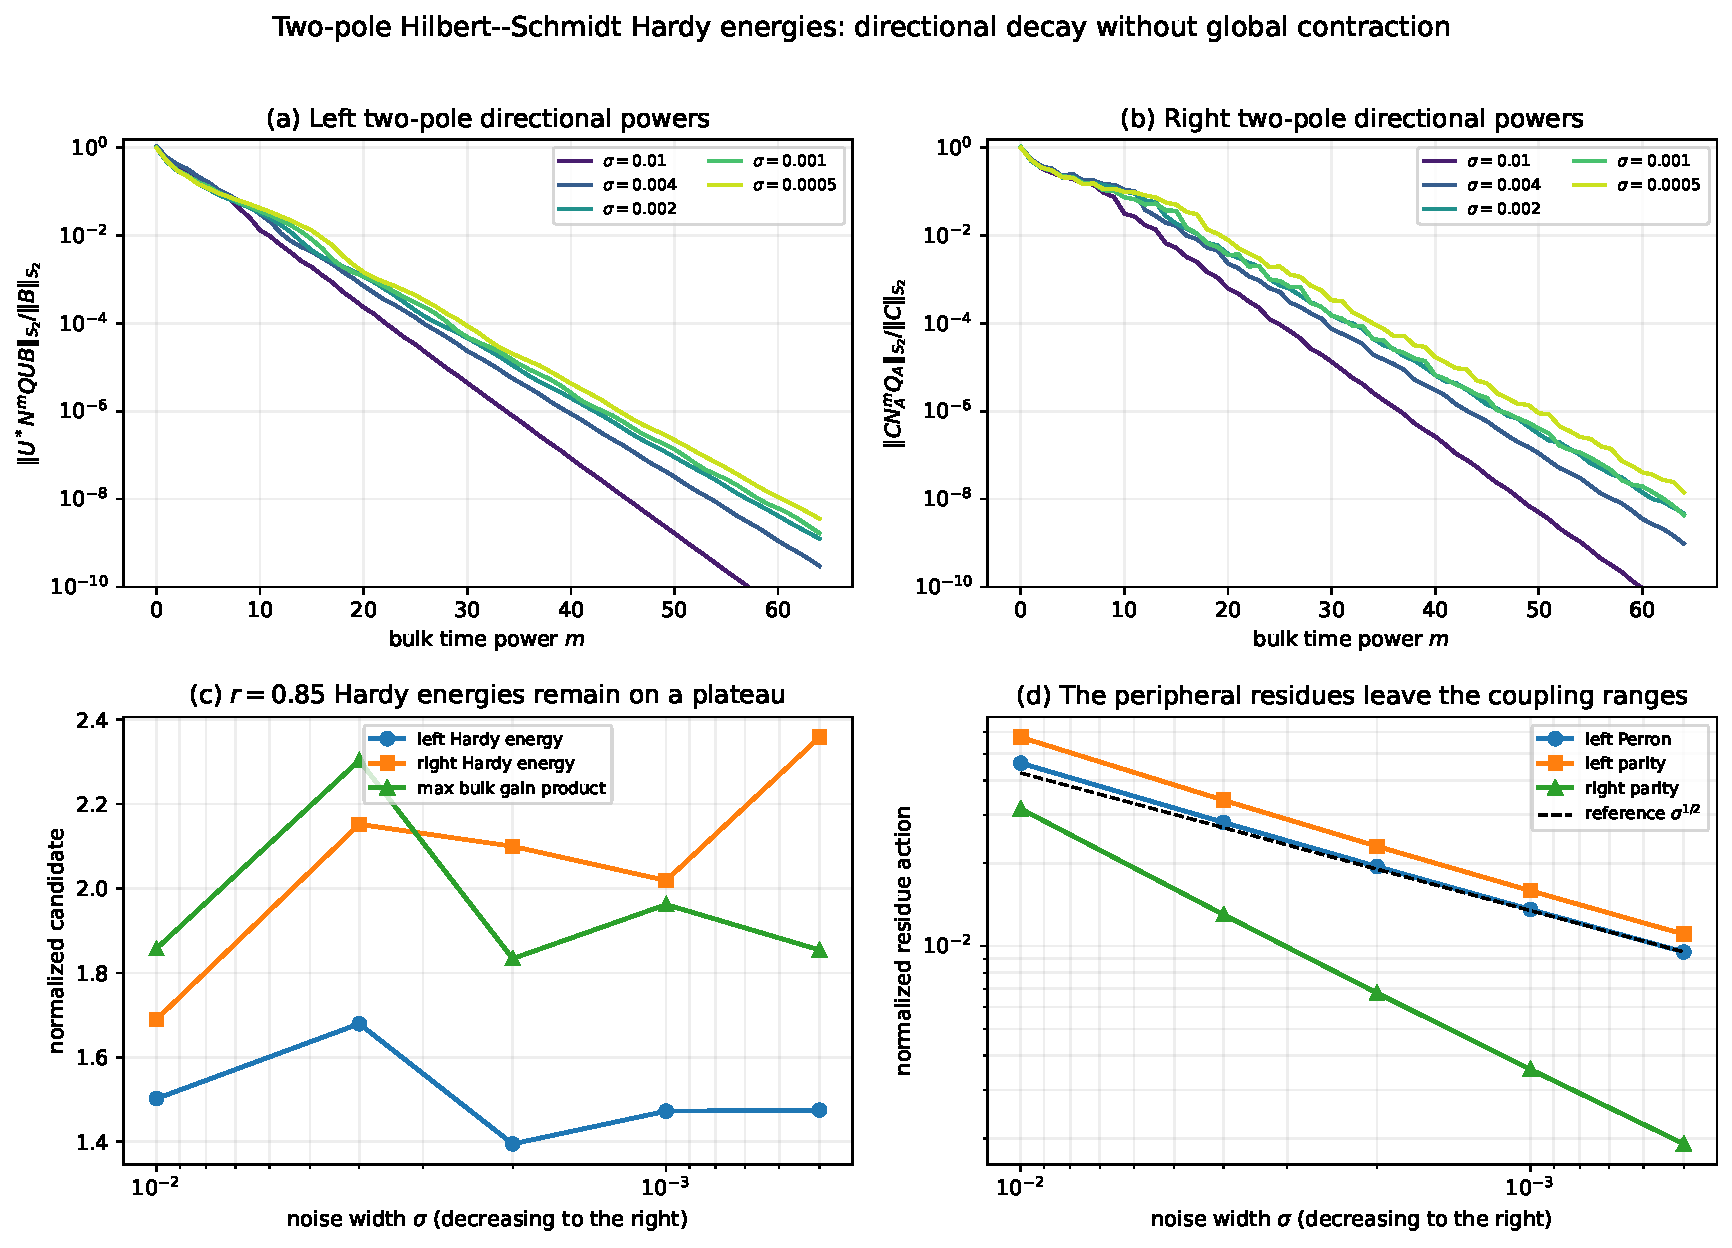
\includegraphics[width=\textwidth]{figures/two_pole_hardy_energy.pdf}
\caption{Two-pole Hardy-energy audit.  (a)--(b) Left and right normalized
bulk powers through time \(64\).  (c) The \(r=0.85\) truncated energies and
the largest direct bulk gain product remain on a narrow five-scale plateau.
(d) Fine Perron/parity and coarse parity residue actions leave the coupling
ranges; the coarse Perron action is an exact algebraic zero and is omitted.}
\label{fig:hardy}
\end{figure}

\subsection{What the computation does and does not say}

The direct contour products in \cref{tab:hardy} use the same truncated
Laurent sums as the power ledger.  The Hardy upper candidates are larger,
between approximately \(3.4\) and \(5.7\) for the separate left/right
actions, because Cauchy--Schwarz intentionally discards phase cancellation.
That loss is acceptable: only a polylogarithmic upper is needed.

Three validation layers remain absent.

\begin{enumerate}[leftmargin=2.2em]
 \item The eight-probe Hutchinson quantities are estimators, not
 deterministic Hilbert--Schmidt uppers.
 \item The tail after \(m=64\) is not enclosed, even though the observed
 decay base lies well below \(r=0.85\).
 \item The sparse hard cutoff, eigenfactors, and bulk radii are not enclosed
 by interval arithmetic at all five scales.
\end{enumerate}

\section{What is proved and the next gate}
\label{sec:boundary}

The current state can be summarized without a global resolvent claim.

\begin{description}[leftmargin=4.2cm,style=nextline]
 \item[Exact operator algebra]
 Two-pole decomposition, Hardy upper, Gramian trace identities, and
 positive Stein supersolution certificates.

 \item[Exact negative result]
 No fixed number of noisy steps can contract the complete stationary
 Perron/parity complement by a noise-uniform factor below one.

 \item[Small-noise analysis]
 The rounded square-root left factors have sharp derivative scale
 \(\Theta(\sigma^{-1})\), the outgoing coupling has two-sided
 Hilbert--Schmidt scale \(\Theta(h\sigma^{-3/2})\), and the exact residue
 block is controlled by the left detail factor.

 \item[Conditional closure]
 Polylogarithmic dyadic Hardy energies and peripheral-factor conditioning
 imply the RH-49 gate and preserve the strict \(n\sigma^2\to\infty\)
 identification range.

 \item[Floating evidence]
 Five-scale power sums, tail fits, direct Laurent products, and residue
 actions through dimension \(40960\).  These are diagnostics, not validated
 asymptotic bounds.
\end{description}

The next paper-level target is therefore concrete: construct positive
low-complexity supersolutions for the left and right Stein equations,
uniformly over dyadic refinement.  A useful candidate should exploit three
features already visible in the data:

\begin{enumerate}[leftmargin=2.2em]
 \item the coupling sources are localized and smoothing;
 \item the two-pole bulk tail decays at a base below \(0.75\) on all stored
 scales;
 \item the deterministic isometric directions are nearly invisible to the
 coupling ranges, even though they prevent global contraction.
\end{enumerate}

A failed Stein ansatz would also be informative: its positive residual
would identify which spatial or temporal sector carries the missing energy.
This is substantially more localized than failure of a global
pseudospectral bound.

\subsection{No arithmetic or Hilbert--P\'olya conclusion}

Every operator in this paper is generated by one explicit noisy quadratic
dynamical system and its cell-average compressions.  The results do not
construct a self-adjoint Hilbert--P\'olya operator, identify an eigenvalue
with a Riemann-zeta zero, prove a prime-power trace formula, derive a
\(T\log T\) counting law, or imply the Riemann hypothesis.  They close one
operator-theoretic reduction and identify the next rigorous certificate
inside the existing spectral program.

\section{Reproducibility}
\label{sec:reproducibility}

The archive contains:

\begin{itemize}[leftmargin=2em]
 \item \path{src/two_pole_hardy}, implementing exact two-pole deflation,
 Hardy bounds, discrete Gramians, and Stein supersolution checks;
 \item \path{experiments/run_two_pole_hardy_pilot.py}, the five-scale
 exact-Haar power and residue audit;
 \item \path{experiments/build_hardy_certificate.py}, composing the analytic
 and floating evidence ledger;
 \item \path{experiments/make_figures.py}, reproducing
 \cref{fig:hardy};
 \item \path{tests}, checking the exact algebra, Hardy inequality, Gramian
 identities, supersolution logic, archived slopes, tail decay, residue
 suppression, and source hashes;
 \item \path{results}, containing the full and smoke pilots, theorem
 certificate, dependency manifest, summary, and archive verification.
\end{itemize}

From this directory, the principal commands are
\begin{verbatim}
PYTHONDONTWRITEBYTECODE=1 /root/math/.venv/bin/pytest -q

OPENBLAS_NUM_THREADS=16 OMP_NUM_THREADS=16 \
PYTHONDONTWRITEBYTECODE=1 /root/math/.venv/bin/python \
  experiments/run_two_pole_hardy_pilot.py

PYTHONDONTWRITEBYTECODE=1 /root/math/.venv/bin/python \
  experiments/build_hardy_certificate.py
MPLBACKEND=Agg PYTHONDONTWRITEBYTECODE=1 /root/math/.venv/bin/python \
  experiments/make_figures.py
latexmk -pdf -interaction=nonstopmode -halt-on-error main.tex
PYTHONDONTWRITEBYTECODE=1 /root/math/.venv/bin/python \
  experiments/build_archive.py
PYTHONDONTWRITEBYTECODE=1 /root/math/.venv/bin/python \
  experiments/verify_archive.py
\end{verbatim}

The full pilot is the expensive step.  Rebuilding the certificate, figure,
tests, manuscript, and archive from the stored full pilot is inexpensive.

\bibliographystyle{plainnat}
\bibliography{references}

\end{document}
